\documentclass{standalone}

\usepackage{tikz}

\usetikzlibrary{positioning, chains, shapes.geometric, fit, shapes, arrows.meta, calc}

\begin{document}

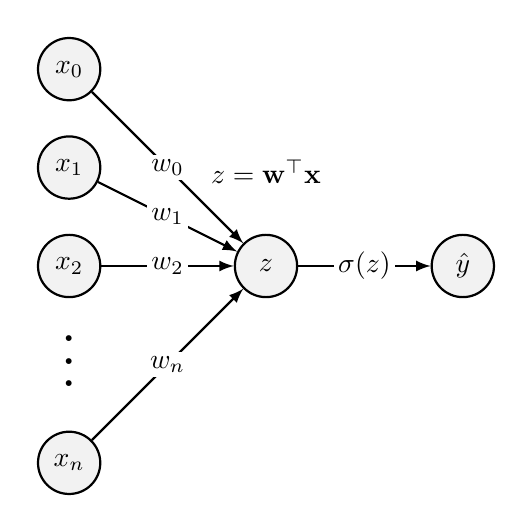
\begin{tikzpicture}[
    >=LaTeX, % Use default LaTeX arrows
    % Styles 
    node/.style={ % Input or output node
        circle,
        minimum width=2.25em,
        draw,
        fill=gray!10,
        thick
    },
    cell/.style={
        rectangle,
        rounded corners=2mm,
        minimum height=2.5em,
        minimum width=2.5em,
        draw,
        thick
    }, 
    arrow/.style={
        -latex,
        thick
    },
    backprop/.style={ % Backpropagation arrows
        arrow,
        dashed,
        gray
    }
]
    
    % The first two x nodes are spaced out more
    \foreach \x in {0,1,2}
        \node[node] (x\x) at (0,-\x*1.25) {$x_{\x}$};
    \node[node] (xm) at (0,-4*1.25) {$x_{n}$};

    % The dots are placed between x2 and xm
    %\node at (0,{-3.4}) {$\vdots$};
    \path (x2) -- (xm) node[pos=0.35, scale=2] {\vdots};

    % The xm node is placed further down to make space for the dots
  
    % Mid Node
    \node[node] (z) at (2.5,-2.5) {$z$};
  
    % Output Node
    \node[node, right of=z, node distance=2.5cm] (yhat) {$\hat{y}$};
    
      % Arrows from input nodes to mid node with labels above
        \draw[arrow] (x0) -- (z) node[midway, fill=white, inner sep=1.5pt] {$w_0$};
        \foreach \x in {1,...,2}
            \draw[arrow] (x\x) -- (z) node[midway, fill=white, inner sep=1.5pt] {$w_{\x}$};
        \draw[arrow] (xm) -- (z) node[midway, fill=white, inner sep=1.5pt] {$w_{n}$};
  
    % Arrow from mid node to output node with sigma(z) over it
    \draw[arrow] (z) -- (yhat) node[midway, fill=white, inner sep=1.5pt] {$\sigma(z)$};
  
    % Equations.
    \node[above of=z, node distance=1.2cm] {$z = \mathbf{w}^\top \mathbf{x}$};

    \node[rectangle, rounded corners=2mm, minimum height=2.5em, minimum width=2.5em, fit=(x0) (xm)] (xbox) {};
\end{tikzpicture}

\end{document}